\section{Prime divisors and weighted zero arcs}
\label{sec:arithmetic}

\subsection{A local valuation inequality}

For a rational number \(u\ne0\), let \(\ord_p(u)\) be its usual
\(p\)-adic valuation, and put \(\ord_p(0)=+\infty\).
We only use primes \(\sqrt n<p\le n\), so a nonzero distance of
absolute value at most \(n\) has valuation at most one.

\begin{lemma}[A coefficientwise divisor]\label{lem:valuation}
For such a prime and an integer \(0\le\ell\le n\), put
\[
w_a(p,\ell)=
\left\lfloor\frac{\ell_a}{p}\right\rfloor
-\left\lfloor\frac{\ell-\alpha_a}{p}\right\rfloor
-\left\lfloor\frac{\beta_a-\ell}{p}\right\rfloor.
\]
Each \(w_a\) is \(0\) or \(1\). Every coefficient of \(x^{n-\ell}\)
in \(A_{h,j,n}\) has valuation at least
\begin{equation}\label{eq:valbound}
\sum_{a=0}^{m}w_a(p,\ell)+j.
\end{equation}
\end{lemma}
\begin{proof}
The assertion \(w_a\in\{0,1\}\) follows from
\(\lfloor u+v\rfloor-\lfloor u\rfloor-\lfloor v\rfloor\in\{0,1\}\),
with \(u=(\ell-\alpha_a)/p\) and \(v=(\beta_a-\ell)/p\).

For a pole factor, the constant in~\eqref{eq:polelocal} is a binomial
coefficient of valuation exactly \(w_a\), by the factorial valuation
formula and \(p^2>n\). Its coefficient of order \(u\) has valuation
at least \(w_a-u\).

For a regular factor the constant term has valuation \(w_a-1\).
For example, if \(\ell<\alpha_a\) and \(s=\alpha_a-\ell\), it equals
\[
H_a(-\ell)=\frac{\ell_a!(s-1)!}{(s+\ell_a)!}.
\]
Use
\(\lfloor(s-1)/p\rfloor=-\lfloor-s/p\rfloor-1\);
the other side of the interval is identical up to sign.
Expansion of the reciprocal linear factors loses at most one
valuation per order, so order \(u\) has valuation at least
\(w_a-1-u\).

The needed total order is at most \(\mu_\ell-1-j\), and there are
\(M-\mu_\ell\) regular factors. Since
\(\ord_p(d_n)=1\), the lower bound after multiplication by \(d_n^m\)
is
\[
m+\sum_aw_a-(M-\mu_\ell)-(\mu_\ell-1-j)
=\sum_aw_a+j.
\]
The factor \(m!/j!\) and coefficients of \((-\ell+w)^h\) are integers
and cannot lower this bound. Sums of terms preserve the lower bound.
\end{proof}

This estimate is stronger than needed. We discard the extra \(j\)
and minimize over the pole location in order to obtain a divisor
common to all entries of the matrix.

\subsection{Replacing pole locations by a circle}

Write \(n=LN_0\). For the grouped intervals define
\begin{equation}\label{eq:W}
W_j(z,y)=\lfloor(L-2t_j)z\rfloor
-\lfloor y-t_jz\rfloor-\lfloor(L-t_j)z-y\rfloor.
\end{equation}
It is periodic in \(z\) and \(y\) with period one and takes values
in \(\{0,1\}\). At \(z=N_0/p,\ y=\ell/p\), it is precisely the
local \(w_a\) for an interval of type \(j\).

For generic \(z\), the set on which \(W_j(z,y)=0\) is the closed
counterclockwise arc from \(\{t_jz\}\) to \(\{(L-t_j)z\}\).
Its length is \(\{(L-2t_j)z\}\), where braces denote fractional part.
Thus
\begin{equation}\label{eq:f}
f(z)=\min_{0\le y<1}\sum_j\nu_jW_j(z,y)
=M-\max_y\{\text{total weight of zero arcs containing }y\}.
\end{equation}
The weights are the interval multiplicities \(\nu_j\).

\begin{figure}[ht]
\centering
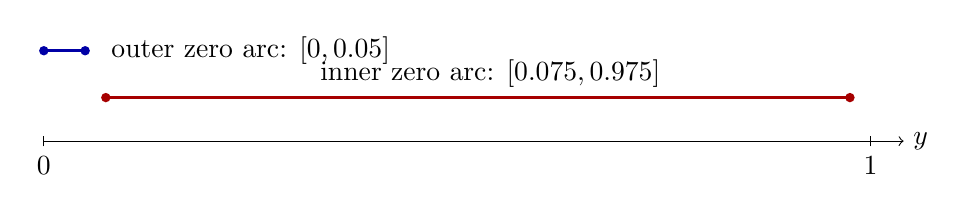
\begin{tikzpicture}[x=10.5cm,y=0.85cm]
\draw[->] (0,0)--(1.04,0) node[right]{\(y\)};
\foreach \x/\lab in {0/0,1/1}
{\draw (\x,-0.08)--(\x,0.08); \node[below] at (\x,-0.08){\(\lab\)};}
\draw[very thick,blue!65!black] (0,1.35)--(0.05,1.35);
\fill[blue!65!black] (0,1.35) circle (1.7pt);
\fill[blue!65!black] (0.05,1.35) circle (1.7pt);
\node[right] at (0.07,1.35){outer zero arc: \([0,0.05]\)};
\draw[very thick,red!65!black] (0.075,0.65)--(0.975,0.65);
\fill[red!65!black] (0.075,0.65) circle (1.7pt);
\fill[red!65!black] (0.975,0.65) circle (1.7pt);
\node[above] at (0.54,0.65){inner zero arc: \([0.075,0.975]\)};
\end{tikzpicture}
\caption{For \(L=14,\ t_0=0,\ t_1=1,\ z=3/40\), the zero arcs
are disjoint. With equal weights \(r\), their common-complement cost
is \(f(z)=r\): at least one type contributes \(r\) at every \(y\).}
\label{fig:arcs}
\end{figure}

All endpoints are affine integer multiples of \(z\), modulo one.
Their cyclic order changes only at the following finite rational set.
Let
\[
\mathcal S=\{0\}\cup\{t_j,L-t_j:0\le j<J\},\qquad
\mathcal D=\{|u-v|:u,v\in\mathcal S,\ u\ne v\}.
\]
Take all fractions \(a/d\in[0,1]\) with \(d\in\mathcal D\), remove
duplicates, and list them as
\[
0=u_0<u_1<\cdots<u_R=1.
\]
On each open interval \((u_r,u_{r+1})\), the integer \(f(z)\) is
constant. At a fixed rational midpoint \(z\), it can be calculated
exactly by checking midpoints between consecutive arc endpoints.
Off this exceptional set no distinct endpoints coincide, so an
endpoint cannot have a smaller value than both adjacent open arcs.

To avoid endpoint conventions entirely, define \(f=0\) at every
breakpoint and extend it periodically. This only weakens the local
divisor estimate and does not change any integral below.

\subsection{The common divisor and its exact exponential rate}

Define
\begin{equation}\label{eq:Pi}
\Pi_n=\prod_{\sqrt n<p\le n}p^{f(N_0/p)}.
\end{equation}
By Lemma~\ref{lem:valuation}, \(\Pi_n\) divides every integer
coefficient of every \(A_{h,j,n}(x)\). It is a rational integer;
we do not need factorization into Gaussian primes.

\begin{proposition}[Digamma formula]\label{prop:gamma}
The limit \(\gamma=\lim n^{-1}\log\Pi_n\) exists and is
\begin{equation}\label{eq:gamma}
\boxed{\displaystyle
\gamma=\frac1L\sum_{\substack{0\le r<R\\u_r>0}}
 f\!\left(\frac{u_r+u_{r+1}}2\right)
 \bigl(\psi(u_{r+1})-\psi(u_r)\bigr),}
\end{equation}
where \(\psi=\Gamma'/\Gamma\).
\end{proposition}
\begin{proof}
For all sufficiently small \(z>0\), none of the endpoints wraps
around the circle and the zero arcs are nested about \(Lz/2\).
They have a common point, so \(f(z)=0\). Thus the apparent singularity
at \(u_0=0\) contributes nothing.

For an interval \((a,b)\subset(0,1)\) on which \(f=v\), periodicity
selects primes satisfying
\[
N_0/(r+b)<p<N_0/(r+a),\qquad r=0,1,\ldots.
\]
For each fixed \(r\), the prime number theorem
\(\vartheta(X)=\sum_{p\le X}\log p=X+o(X)\) makes their contribution
to \(n^{-1}\log\Pi_n\) tend to
\[
\frac vL\left(\frac1{r+a}-\frac1{r+b}\right).
\]
The sum over \(r\ge T\) is bounded, uniformly in large \(n\), by a
constant times \(M/(LT)\), using the elementary Chebyshev bound
\(\vartheta(X)=O(X)\). Primes below \(\sqrt n\) contribute \(o(n)\).
These observations justify passage from finitely many periods to all
periods.

Breakpoint exclusions also cost only \(O(\log n)\). Indeed,
\(\{N_0/p\}=a/d\) implies that \(p\) divides \(dN_0\);
the denominators \(d\) belong to a fixed finite set.
Finally,
\[
\sum_{r=0}^{\infty}
\left(\frac1{r+a}-\frac1{r+b}\right)=\psi(b)-\psi(a).
\]
Summing over the finite partition proves the formula.
\end{proof}

The formula is a lower bound on the content available for division,
not a formula for the entire actual gcd of a row after evaluation
at \(x=\ii\). Additional cancellations at \(\ii\) could give more
divisibility.

\subsection{A transparent two-layer special case}

For \(t_0=0,t_1=1\) with weights \(r,M-r\), put
\[
a_\ell=\max\left(\frac{\ell}{L},\frac{\ell-1}{L-2}\right),
\qquad b_\ell=\frac{\ell}{L-1},
\quad 1\le\ell\le L-2.
\]
On these intervals the two zero arcs are disjoint, and
\(f=\min(r,M-r)\). They are precisely the disjointness intervals
away from endpoints. Hence
\begin{equation}\label{eq:twogamma}
\gamma=\frac{\min(r,M-r)}L
\sum_{\ell=1}^{L-2}\bigl(\psi(b_\ell)-\psi(a_\ell)\bigr).
\end{equation}
This is a useful small test of the general partition algorithm.
For many layers, the weighted maximum-overlap calculation is more
effective than checking pairwise disjointness alone.
